\documentclass{article}

\usepackage[ngerman]{babel}										% Statt german, \autoref zeigt damit "Abbildung x" an
\usepackage{graphicx}											% Graphiken einbinden
\usepackage[left=3cm,right=3cm,top=3cm,bottom=3cm]{geometry}	% Abstände zu den Papierrändern
\usepackage[utf8]{inputenc}										% Zeichenkodierung
\usepackage{mathtools}											% Stellt Mathe-Umgebung bereit
\usepackage{float}												% Improves floating elements
\usepackage{lmodern}											% Andere Schriftart (bessere Druckbarkeit)
\usepackage{pdfpages}											% Einbinden von PDF-Dokumenten
\usepackage{fancyhdr}											% Fancy Headers / Footers
\usepackage{listliketab}										% Lists with tab stops
\usepackage{setspace}											% Anpassung von Zeilenabständen
\usepackage{siunitx}											% Korrekte Darstellungen von Einheiten (\SI{1.5}{\milli\volt})
\usepackage{hyperref}   										% Objekte referenzieren (\autoref)
\usepackage{subcaption}
\usepackage{listings}
\usepackage{tikz}
\usepackage{etoolbox} %for making filenames as captions for figures

\makeatletter%for making filenames as captions for figures
\patchcmd{\Gin@setfile}% <cmd>
  {\ProvidesFile}% <search>
  {\xdef\imgfilename{#3}\ProvidesFile}% <replace>
  {}{}% <success><failure>
\makeatother

% dark mode
%\usepackage{xcolor}			
%\pagecolor[rgb]{0,0,0}
%\color[rgb]{1,1,1}

\setlength{\parindent}{0em}										% Keine Einrückung bei Absatzbeginn
\setlength{\parskip}{1em}										% Dafür vert. Abstand zw. Absätzen

\renewcommand{\arraystretch}{1.2}								% Verzeichnisse kompakter darstellen

\newcommand{\tbf}{\textbf}										% Shortcut für fetten Text

\makeatletter
\g@addto@macro\bfseries{\boldmath}								% \mathbf nicht im Inhaltsverzeichnis darstellen
\makeatother

\pagestyle{fancy}												% Benutzung von fancyhdr
\sisetup{
	locale = DE,
	per-mode=fraction,
	fraction-function=\tfrac,
	binary-units = true
	}

\DeclareSIUnit{\belmilliwatt}{Bm}
\DeclareSIUnit{\dBm}{\deci\belmilliwatt}

\DeclareSIUnit{\belcarrier}{Bc}
\DeclareSIUnit{\dBc}{\deci\belcarrier}

\DeclareSIUnit{\belvolt}{BV}
\DeclareSIUnit{\dBV}{\deci\belvolt}

\DeclareSIUnit{\Bit}{Bit} % bits 

\usepackage{xcolor} %custom colors for code
\definecolor{codegreen}{rgb}{0,0.6,0}
\definecolor{codegray}{rgb}{0.5,0.5,0.5}
\definecolor{codepurple}{rgb}{0.58,0,0.82}
\definecolor{codeblue}{rgb}{0,0,0.92}
\definecolor{backcolour}{rgb}{0.95,0.95,0.92}
\lstdefinestyle{codestyle}{
    backgroundcolor=\color{backcolour},   
    commentstyle=\color{codegreen},
    keywordstyle=\color{codeblue},
    numberstyle=\color{magenta},
    stringstyle=\color{codepurple},
    basicstyle=\ttfamily\footnotesize,
    breakatwhitespace=false,         
    breaklines=true,                 
    captionpos=b,                    
    keepspaces=true,                 
    numbers=left,                    
    numbersep=5pt,                  
    showspaces=false,                
    showstringspaces=false,
    showtabs=false,                  
    tabsize=2
}

\lstset{style=codestyle}
\lhead{}
\rhead{}

% anpassen!
\chead{Grundlagen der Nachrichtentechnik - Praktikum 3}
\lfoot{04.05.2020}
\cfoot{Loïc Fernau, Niklas Bammann}


\rfoot{Seite \thepage}

\usepackage{titlesec}
\titlespacing\section{0pt}{12pt plus 4pt minus 2pt}{0pt plus 2pt minus 2pt}
\titlespacing\subsection{0pt}{0pt}{0pt}
\titlespacing\subsubsection{0pt}{12pt plus 4pt minus 2pt}{0pt plus 2pt minus 2pt}


\begin{document}
	% Titelseite anpassen
	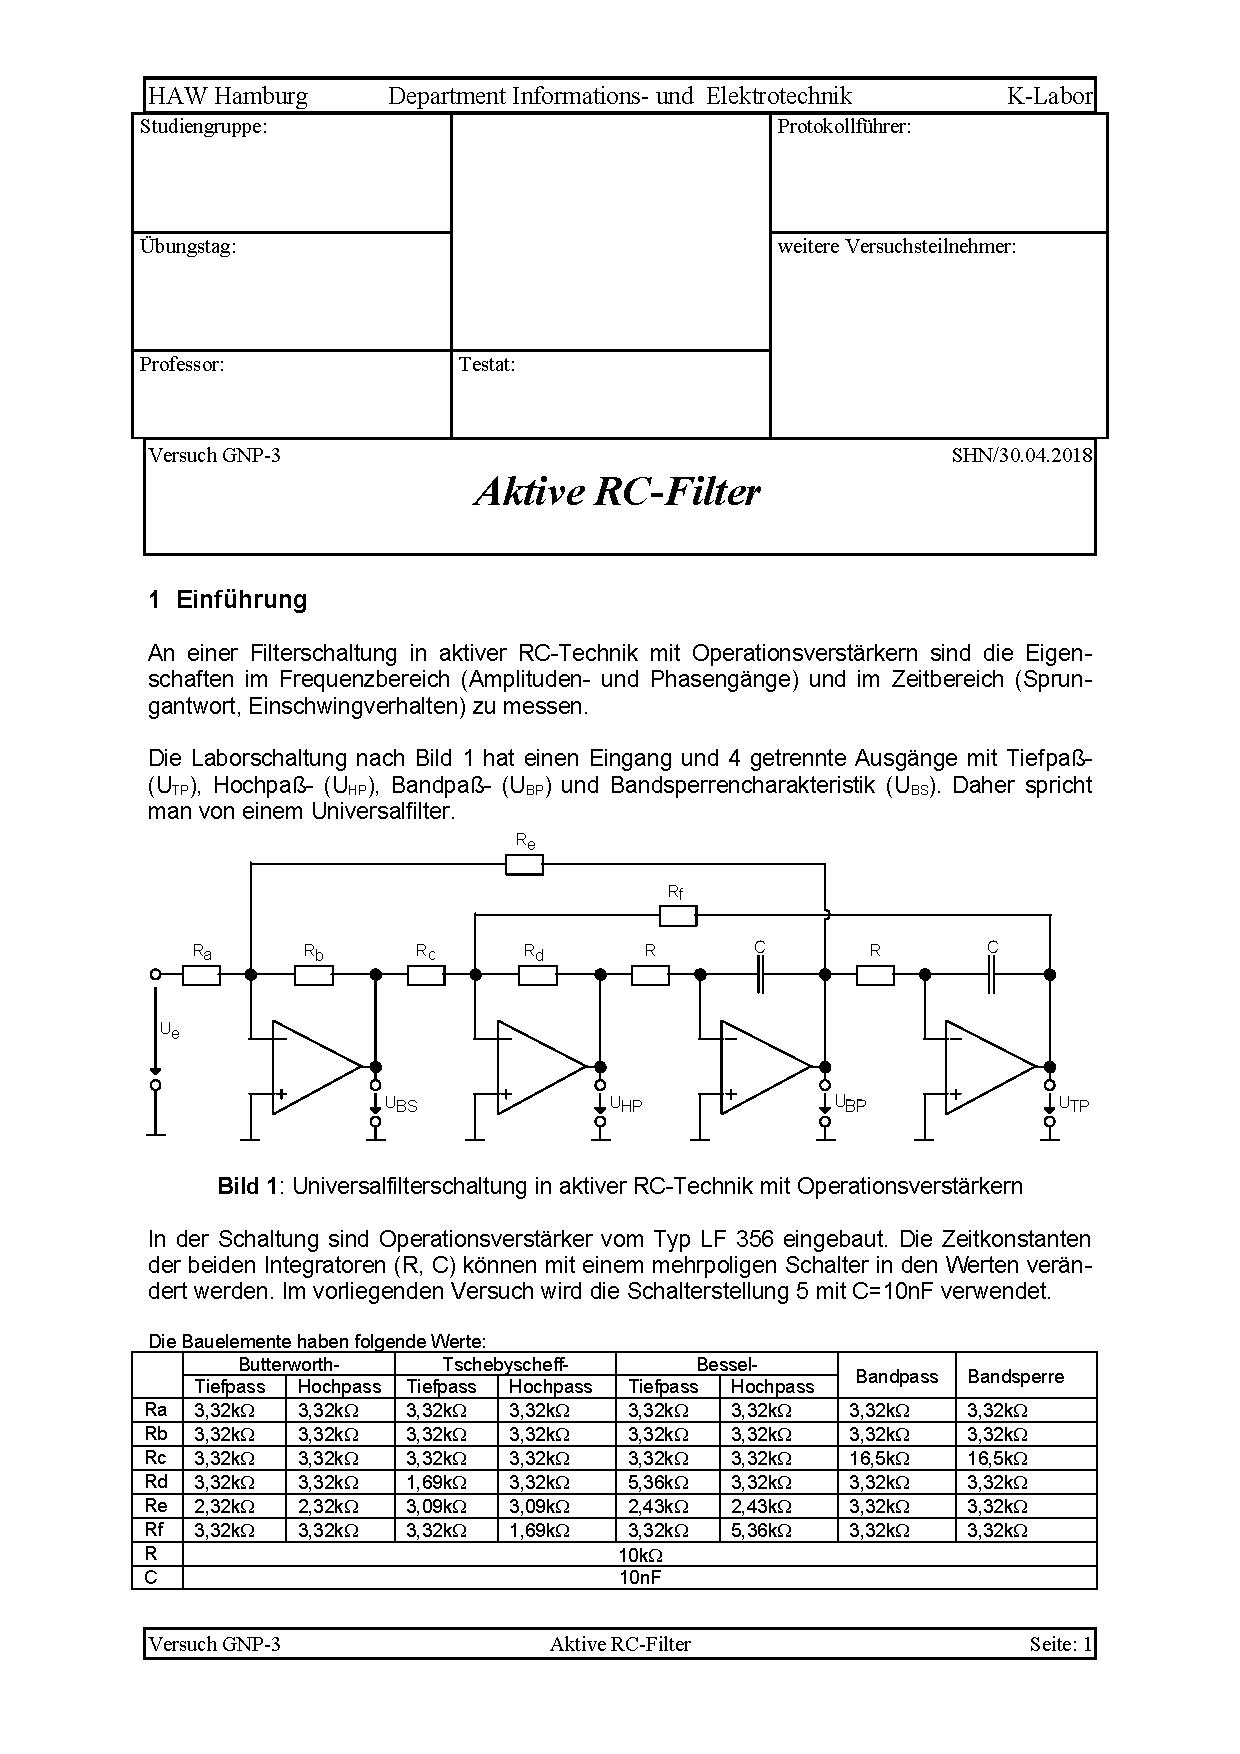
\includepdf[pages=-]{pdf_ext/GNP3_Aktive_RC-Filter.pdf}

 	\begin{titlepage}
 		\begin{flushright}
			
\includegraphics[width=0.5\textwidth]{img/title.png}\\[2cm]
		\end{flushright}
		
		\begin{center}
			%\textsc{\LARGE Hochschule für angewandte Wissenschaften}\\[0.2cm]
			%\textsc{\LARGE Hamburg}\\[1.5cm]
			\textsc{\Large Grundlagen der Nachrichtentechnik}
			\rule{\linewidth}{0.5mm}\\[1.5cm]
			{ \huge \bfseries Praktikumsprotokoll}
			\rule{\linewidth}{0.5mm}\\[2cm]
			% Termin anpassen
			{ \huge \bfseries Aktive RC-Filter}\\[2cm]

			\LARGE Loïc Fernau \\
			\LARGE Niklas Bammann \\[4cm]
			% Gruppe anpassen
			\large GNP
		\end{center}
	\end{titlepage}
	\newpage
	
	\renewcommand{\baselinestretch}{0.8}\normalsize
	\tableofcontents
	\listoffigures
	\listoftables
	\renewcommand{\baselinestretch}{1.0}\normalsize
	
	\newpage

	\setlength{\headsep}{0.4em}
	

	\section{Einleitung}

In diesem Versuch werden die Eigenschaften von aktiven Filterschaltungen untersucht. Dazu werden eine Reihe von Messungen an einem Universalfilter durchgeführt. Zunächst werden Amplituden- und Phasengänge der einzelnen Filterschaltungen numerische berechnet und anschließend messtechnisch aufgezeichnet. Weiterhin werden Sprungantworten der verschiedenen Tiefpässe aufgezeichnet. 

\subsection{Verwendete Geräte}

Für den Versuch weden folgende Geräte verwendet:

\begin{table}[ht]
    \centering
    \begin{tabular}{|c|c|c|c|}\hline
    \tbf{Gerätetyp}     & \tbf{Bezeichnung}         \\ \hline
    Audioanalyzer       & Rohde \& Schwartz UPV     \\ \hline
    Universalfilter     & K-Labor                   \\ \hline
    Oszilloskop         & Tektronix TDS 3014C       \\ \hline
    \end{tabular}
    \caption{Auflistung der Geräte}
\end{table}

	\section{ Vorausberechnung der Schaltung}

Folgende Eigenschaften der Filter sind in häuslicher Vorarbeit zu bestimmen und zum Praktikumstermin vorzulegen:
\subsectio{Grundverstärkung und Grenzfrequenzen der Hoch- und Tiefpässe }
\subsectio{Mittenfrequenz und Bandbreite des Bandpasses }
\subsectio{Sperrfrequenz der Bandsperre }
\subsectio{Übertragungsfunktionen mit Matlab symbolisch berechnet }
\subsectio{Übertragungsfunktionen (Betrag und Phase) mit Matlab numerisch berechnet} 
\subsectio{Spice Simulationsergebnisse für das Frequenzverhalten (AC-Analyse)}

Die Eigenschaften 1-3) können entweder berechnet (siehe Abschnitte 6 und 7) oder aus Simulationen mit Spice (z.B. PSpice oder LTSpice) entnommen werden. Der Berechnungsgang bzw. Schaltung und Plot der Spice-Simulation sind zum Labortermin vorzulegen und in das Protokoll mit aufzunehmen, genauso wie der Matlab-Code.


\subsection{Aufbau}


%%%%%%%%%%%%%%%%%%%%%%%%%%%%%%%%%%%%%%%%%%%%%%%%Comments
%zu 2 :Formeln bzw. Spice-Plots und Ergebnisse der Vorausberechnung für Grundverstärkung und Grenzfrequenzen der Hoch- und Tiefpässe, Mittenfrequenz und Bandbreite des Bandpasses, Sperrfrequenz der Bandsperre. 
	\section{ Messung von Amplituden- und Phasengang der Filterschaltungen }
In diesem Teil sollen die Amplituden und Phasengänge der Filter gemessen und aufgezeichnet werden.
Der hierfür verwendete Universalfilter wurde in der Vorbereitung analysiert.


\subsection*{Aufbau}
Der Universalfilter wird wie im Blockschaltbild an den Audioanalyzer angeschlossen.
Am Audioanalyzer wird das Program "AktFilt Ampl & Phase.set" gestartet und ausgeführt.

% grafik einbinden
\begin{figure}[H]
    \begin{center}
        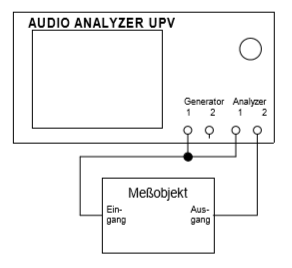
\includegraphics[width=0.5\textwidth]{img/Blockschalt.PNG}
        \caption{Blockschaltbild, Quelle: "GNP3 Aktive RC-Filter.pdf" }
        \label{fig:A3_label}
    \end{center}
\end{figure}






\subsection{Amplituden und Phasengängen von Butterworth-, Tschebyscheff- und Bessel-Tiefpass, logarithmischer}
Die Messung wird mit einem Frequenz "Sweep" von $\SI{100}{\hertz}-\SI{20}{\kilo\hertz}$ durchgeführt.
% grafik einbinden
\begin{figure}[H]
    \begin{center}
        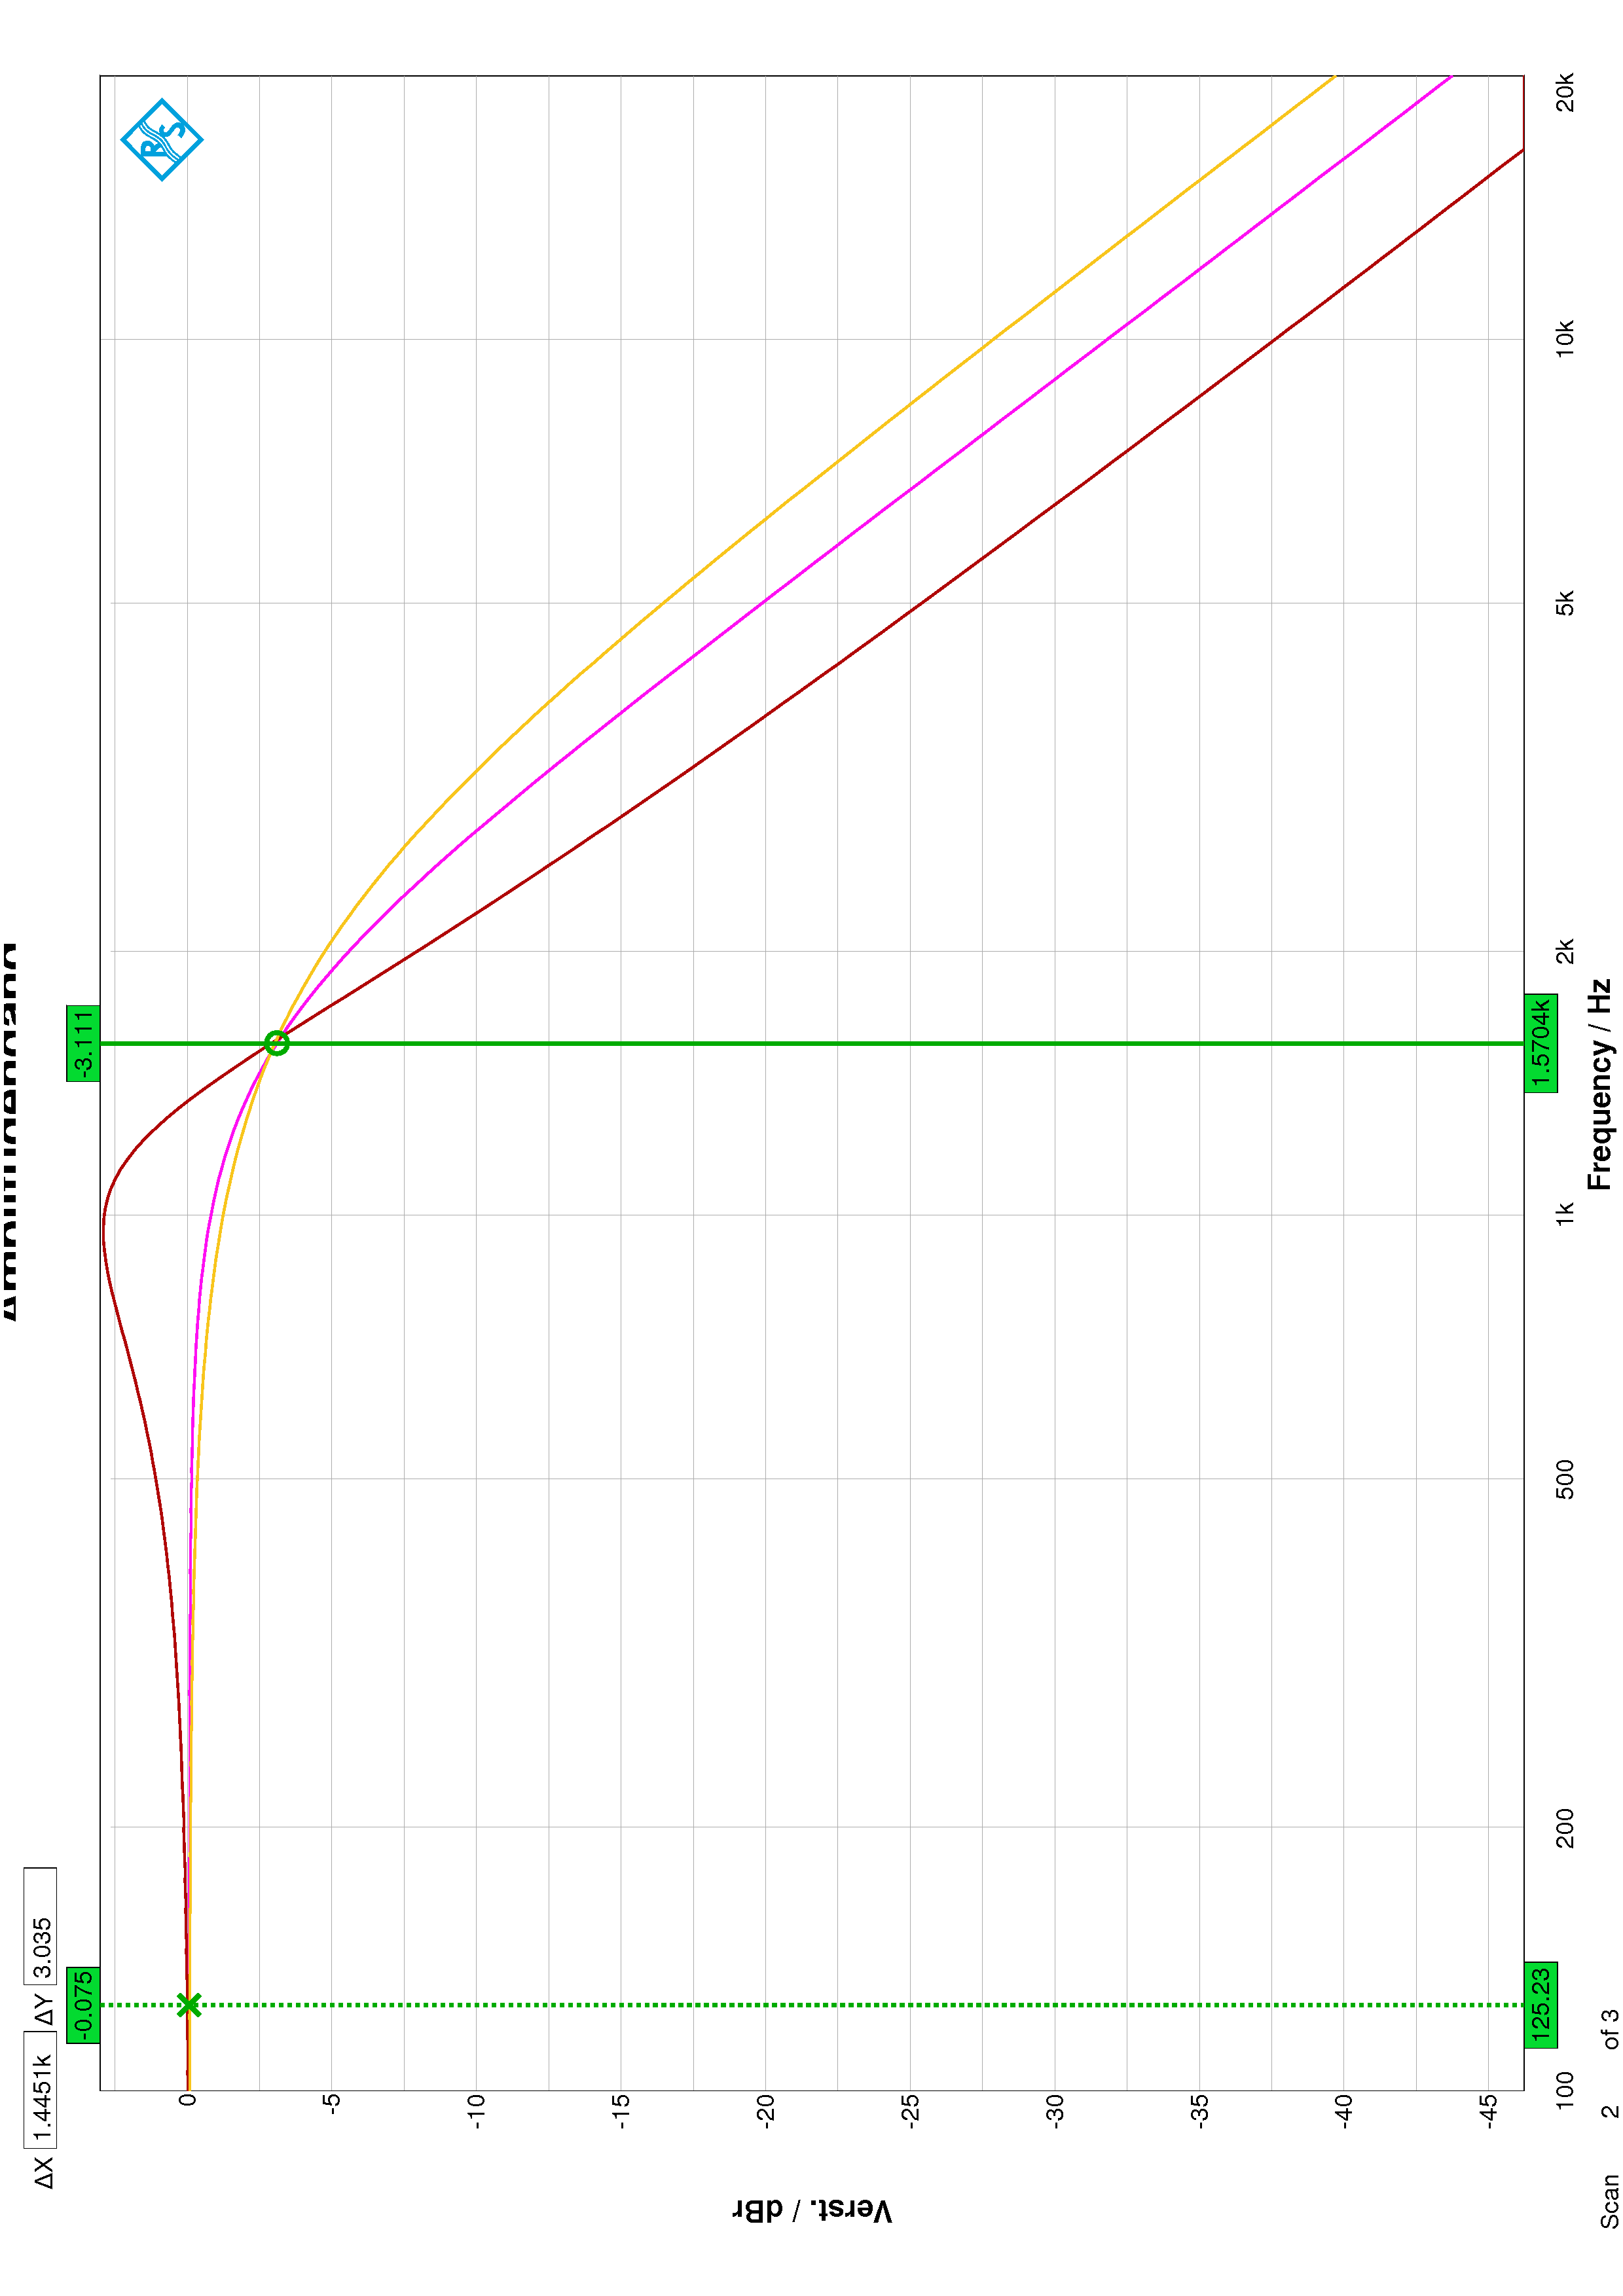
\includegraphics[width=0.8\textwidth, angle =-90]{img/3.1 Amplitudengang.png}
        \caption{Amplitudengang, Rot = Tschebyscheff, Pink = Butterworth , Gelb = Bessel}
        \label{fig:A3_amp}
    \end{center}
\end{figure}
Der Tschebyscheff filter  (Rote Linie) ist leicht an seinem deutlichem über schwingen kurz vor der Grenzfrequenz und schärfsten Abfall der Amplitude zu erkennen. Der Butterworth filter (Pinke Linie) ist der Filter der eine möglichst flache Kurve im Durchlassbereich aufweist. Bleibt noch der Bessel filter (Gelbe Linie) mit seinem geringem über schwingen.

% grafik einbinden
\begin{figure}[H]
    \begin{center}
        \includegraphics[width=0.8\textwidth, angle =-90]{img/3.1 Phasengänge.png} 
        \caption{Phasengänge, Rot = Tschebyscheff, Pink = Butterworth , Gelb = Bessel}
        \label{fig:A3_phase}
    \end{center}
\end{figure}

Aus den Messungen lassen sich die Grenzfrequenzen und Phasen der drei Filter ablesen:
\begin{table}[ht]
    \centering
    \begin{tabular}{|c|c|c|c|}\hline
    \tbf{Filter} & \tbf{Grenzfrequenz $f_g$} & \tbf{Phase $\SI{-60}{\degree}$}     &  \tbf{Phase $\SI{-120}{\degree}$}      \\ \hline
    Butterworth                   & \SI{1570.4}{\hertz} &     \SI{1069.2}{} &\SI{2417.2}{}     \\
    Tschebyscheff             & \SI{1582.6}{\hertz}  &   \SI{915.3}{}  &\SI{1425.2}{}    \\ 
    Bessel                &\SI{1582.6}{\hertz}   &\SI{1248.9}{}&\SI{3298.2}{}  \\ \hline
    \end{tabular}
    \caption{Filter Parameter}
\end{table}




\subsection{Phasengänge von Butterworth-, Tschebyscheff- und Bessel-Tiefpass gemeinsam in einem Plot über linearer Frequenzachse, Frequenzbereich 100Hz...4kHz. }


\begin{table}[ht]
    \centering
    \begin{tabular}{|c|c|c|c|}\hline
    \tbf{Filter} & \tbf{Grenzfrequenz $f_g$} & \tbf{Phase $\SI{-60}{\degree}$}     &  \tbf{Phase $\SI{-120}{\degree}$}     \\ \hline
    Butterworth                   & \SI{1584.6}{\hertz} &     \SI{1251.3}{} &\SI{3283.9}{}     \\
    Tschebyscheff             & \SI{1578.9}{\hertz}  &   \SI{914.6}{}  &\SI{1419.8}{}    \\ 
    Bessel                &\SI{1584.6}{\hertz}   &\SI{1066.4}{}&\SI{2404.5}{}  \\ \hline
    \end{tabular}
    \caption{Grenzfrequenzen der Filter}
\end{table}

% grafik einbinden
\begin{figure}[H]
    \begin{center}
        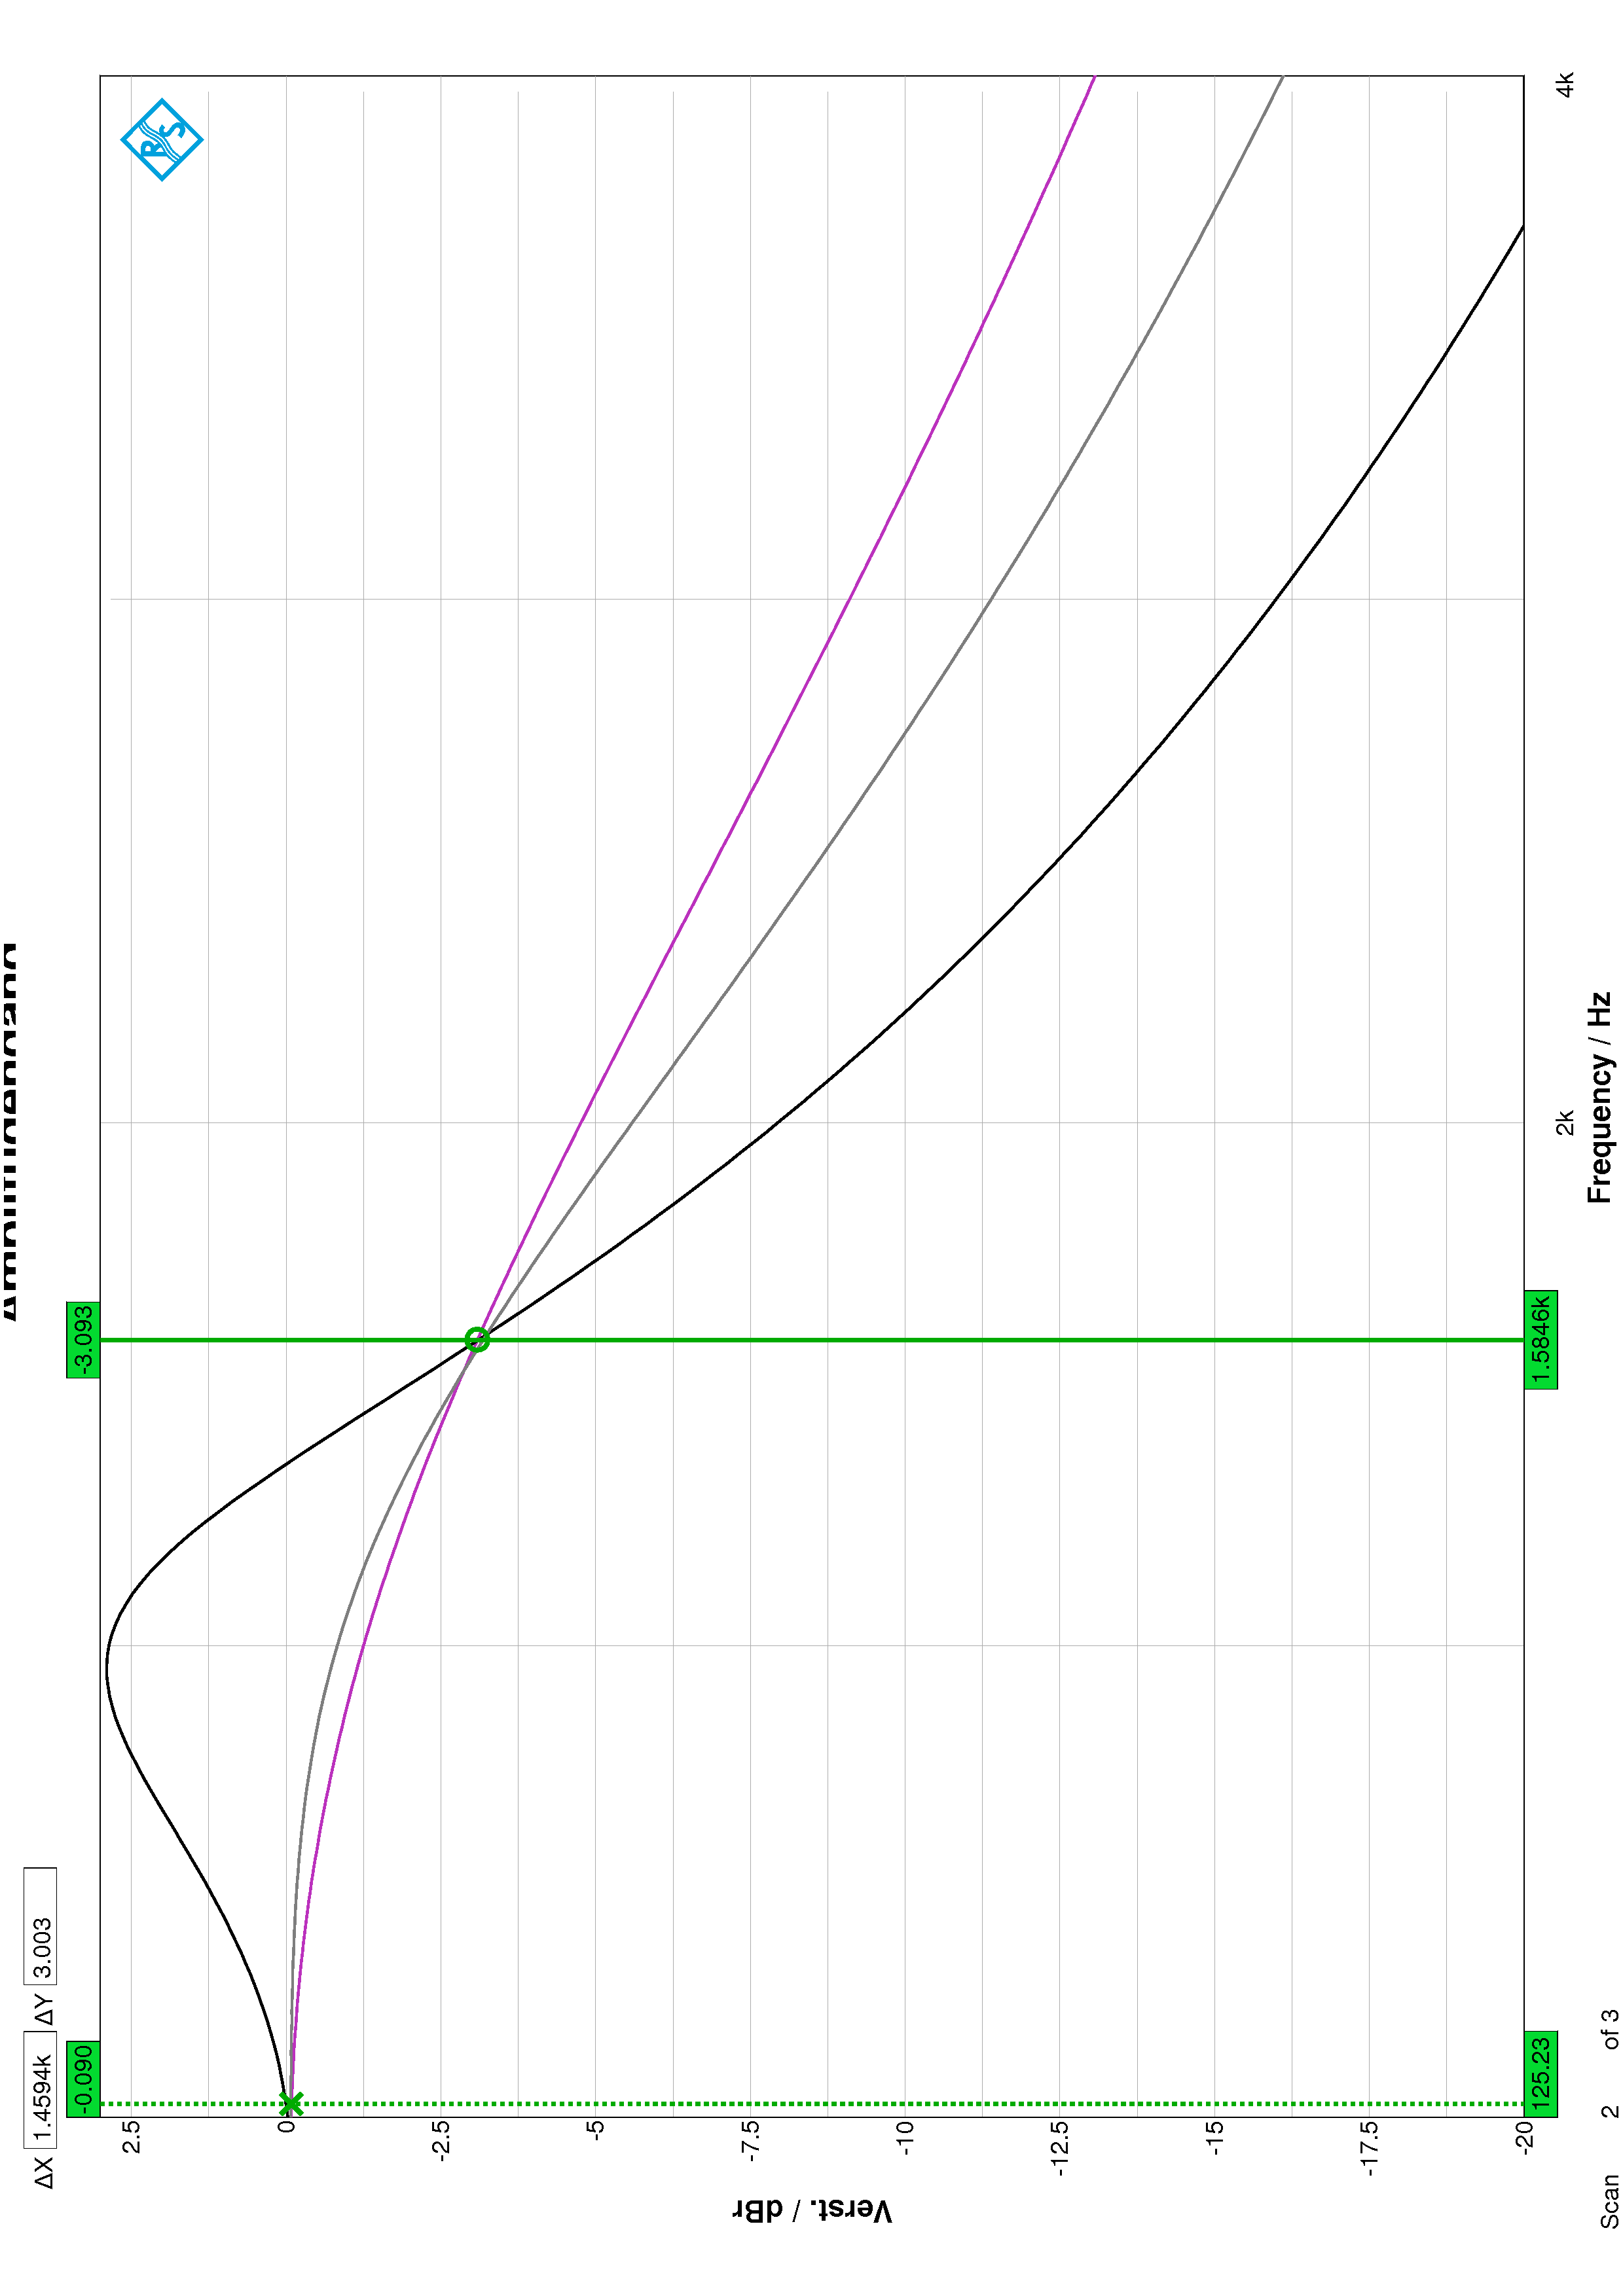
\includegraphics[width=0.8\textwidth, angle =-90]{img/3.2 Amplitudengang linear.png}
        \caption{Amplitudengang linear}
        \label{fig:A3_amp}
    \end{center}
\end{figure}
+

% grafik einbinden
\begin{figure}[H]
    \begin{center}
        \includegraphics[width=0.8\textwidth, angle =-90]{img/3.2 Phasengänge linear.png}
        \caption{Phasengänge linear}
        \label{fig:A3_phase}
    \end{center}
\end{figure}






\subsection{Amplitudengänge (mit Phasengängen) von Butterworth-, Tschebyscheff- und BesselHochpass gemeinsam in einem Plot über logarithmischer Frequenzachse, Frequenzbereich 100Hz...20kHz. }


\begin{table}[ht]
    \centering
    \begin{tabular}{|c|c|c|c|}\hline
    \tbf{Filter}     & \tbf{Grenzfrequenz $f_g$}  \\ \hline
    Butterworth                   & \SI{1632.5}{\hertz}            \\
    Tschebyscheff             & \SI{1607.3}{\hertz}           \\ 
    Bessel                &\SI{1619.8}{\hertz}     \\ \hline
    \end{tabular}
    \caption{Grenzfrequenzen der Filter}
\end{table}

% grafik einbinden
\begin{figure}[H]
    \begin{center}
        \includegraphics[width=0.8\textwidth, angle =-90]{img/3.3 Amplitudengänge HP log.png}
        \caption{\imgfilename}
        \label{fig:A3b_label}
    \end{center}
\end{figure}

% grafik einbinden
\begin{figure}[H]
    \begin{center}
        \includegraphics[width=0.8\textwidth, angle =-90]{img/3.3 Phasengänge HP log.png}
        \caption{\imgfilename}
        \label{fig:A3c_label}
    \end{center}
\end{figure}





\subsection{Amplitudengänge (mit Phasengängen) von Bandpass und Bandsperre gemeinsam in einem Plot über logarithmischer Frequenzachse, Frequenzbereich 1kHz...2,5kHz. }
 

%multi figure
\begin{figure}[H]
\begin{center}
\subfloat[Amplitudengang Bandpass]{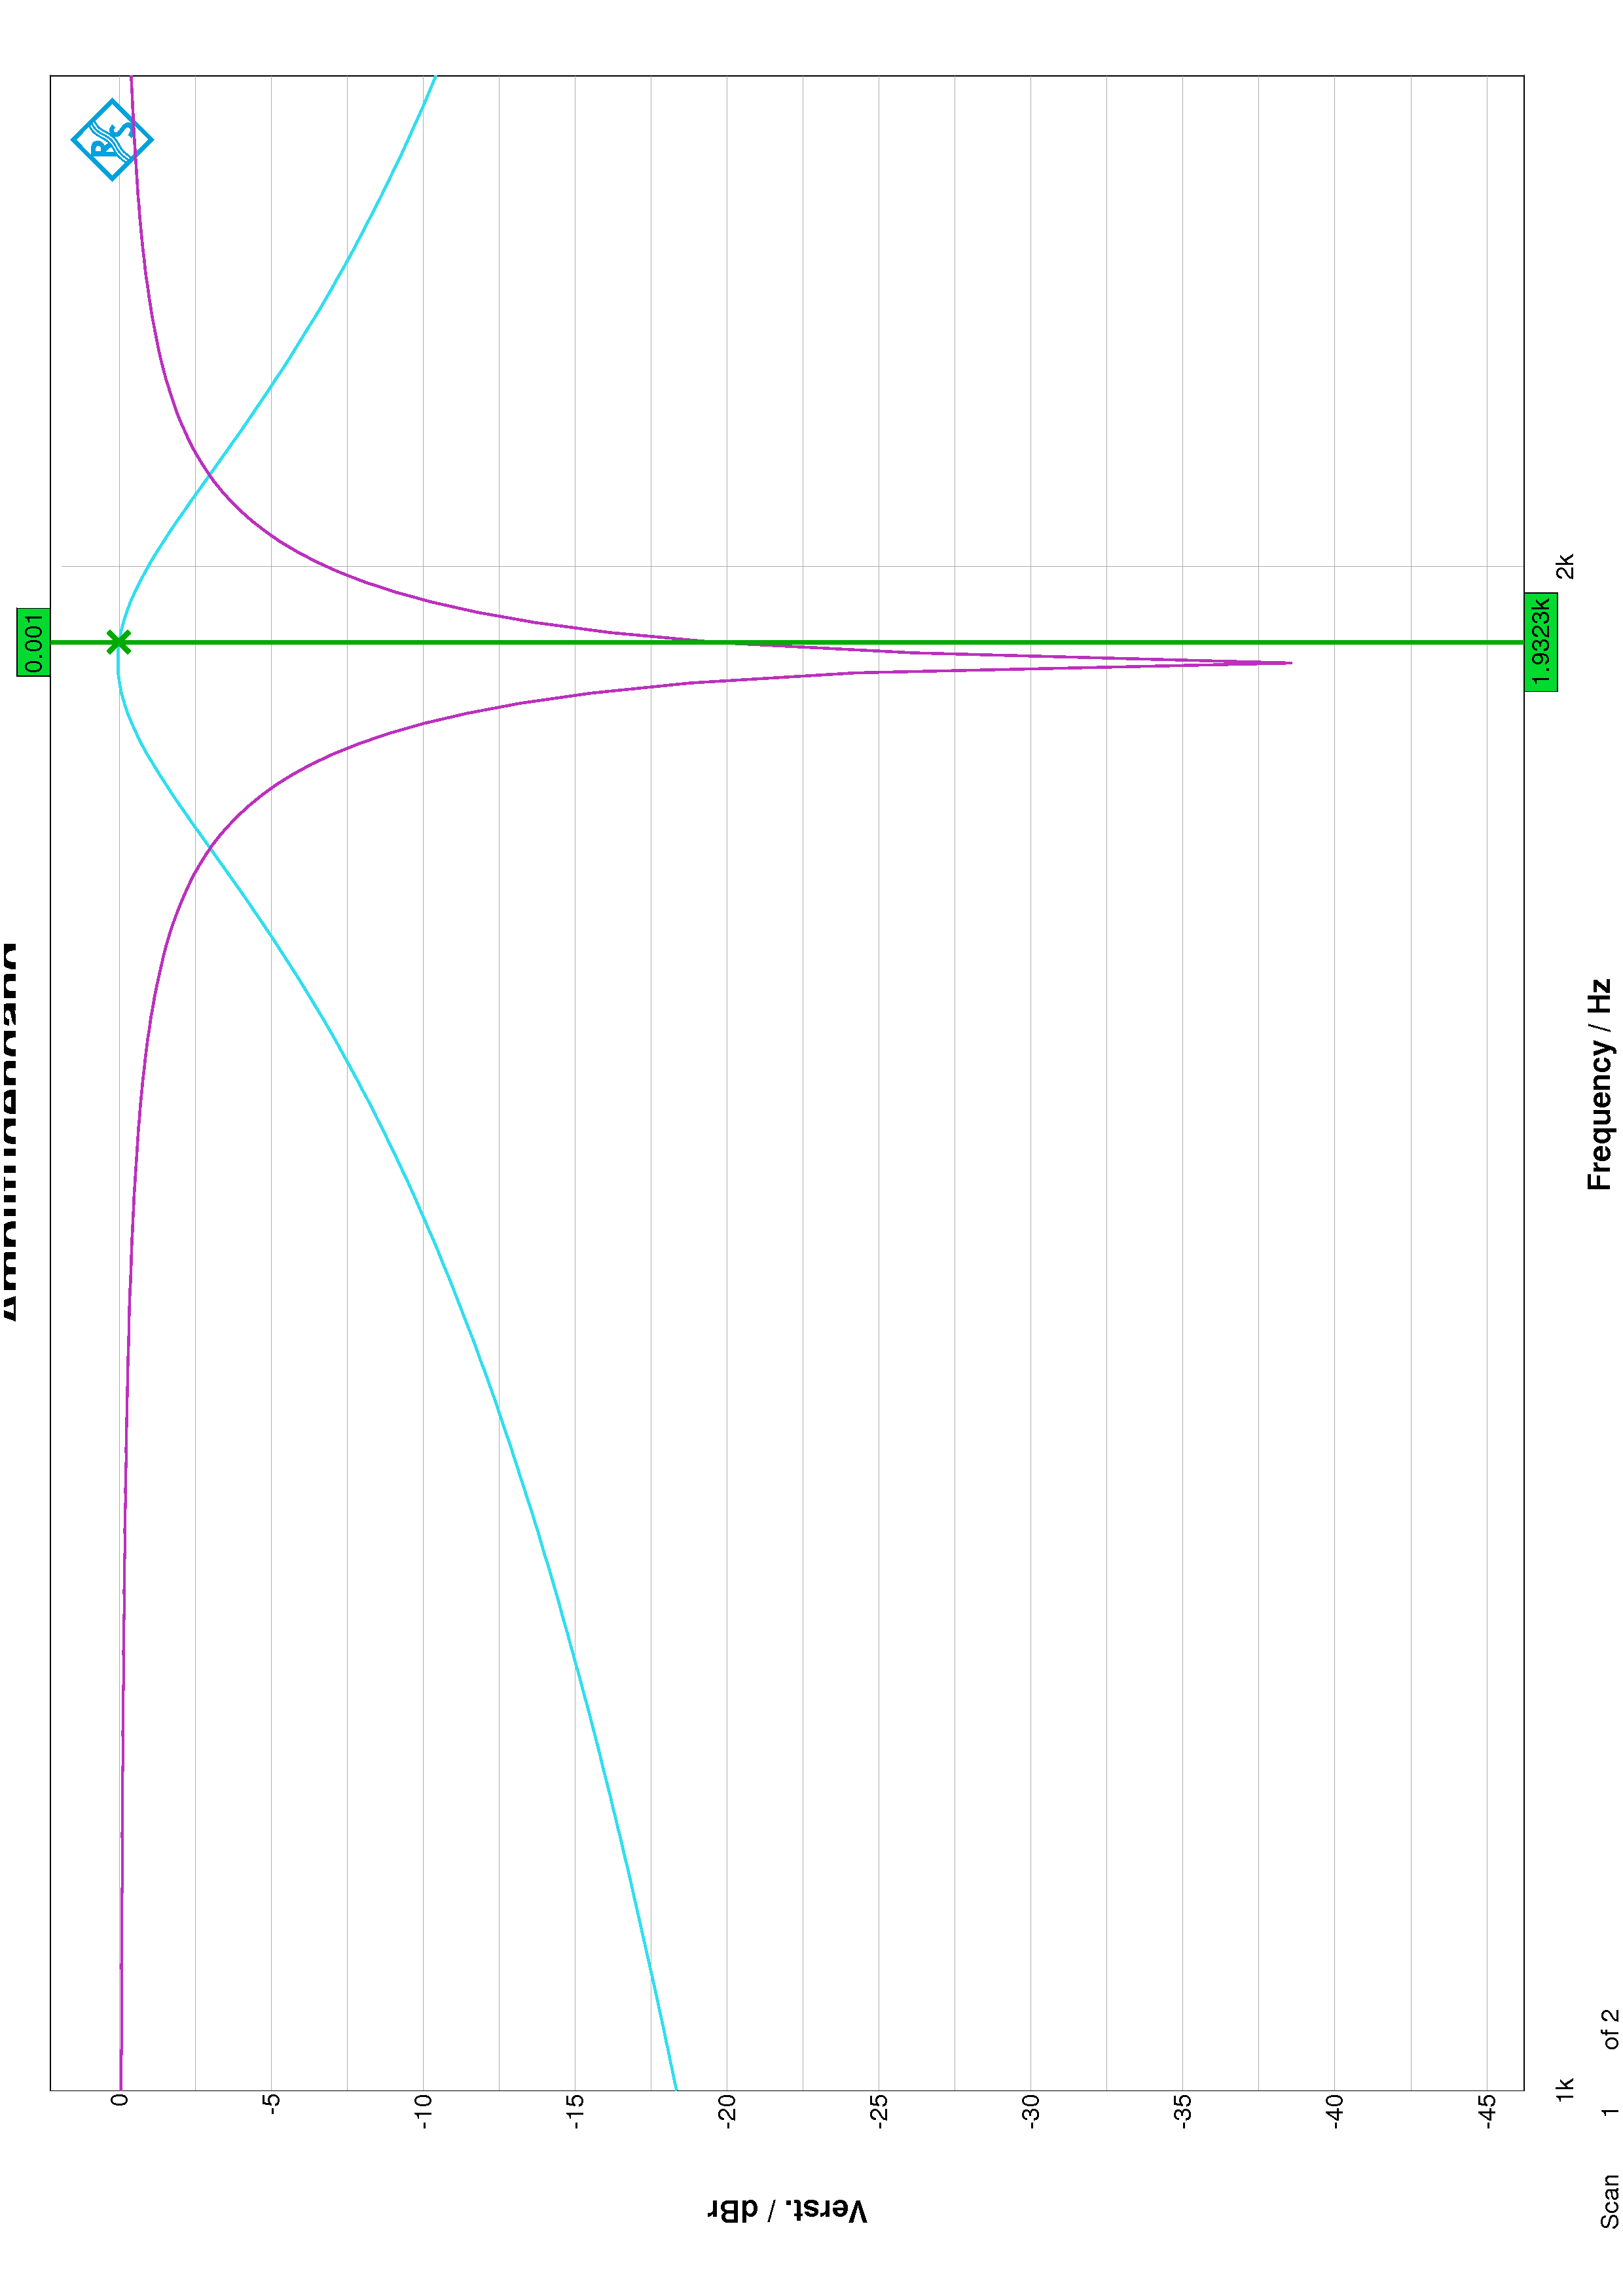
\includegraphics[width = \textwidth/3, angle =-90]{img/3.4 Amplitudengang Bandpass.png}}  
\subfloat[Amplitudengang Bandsperre]{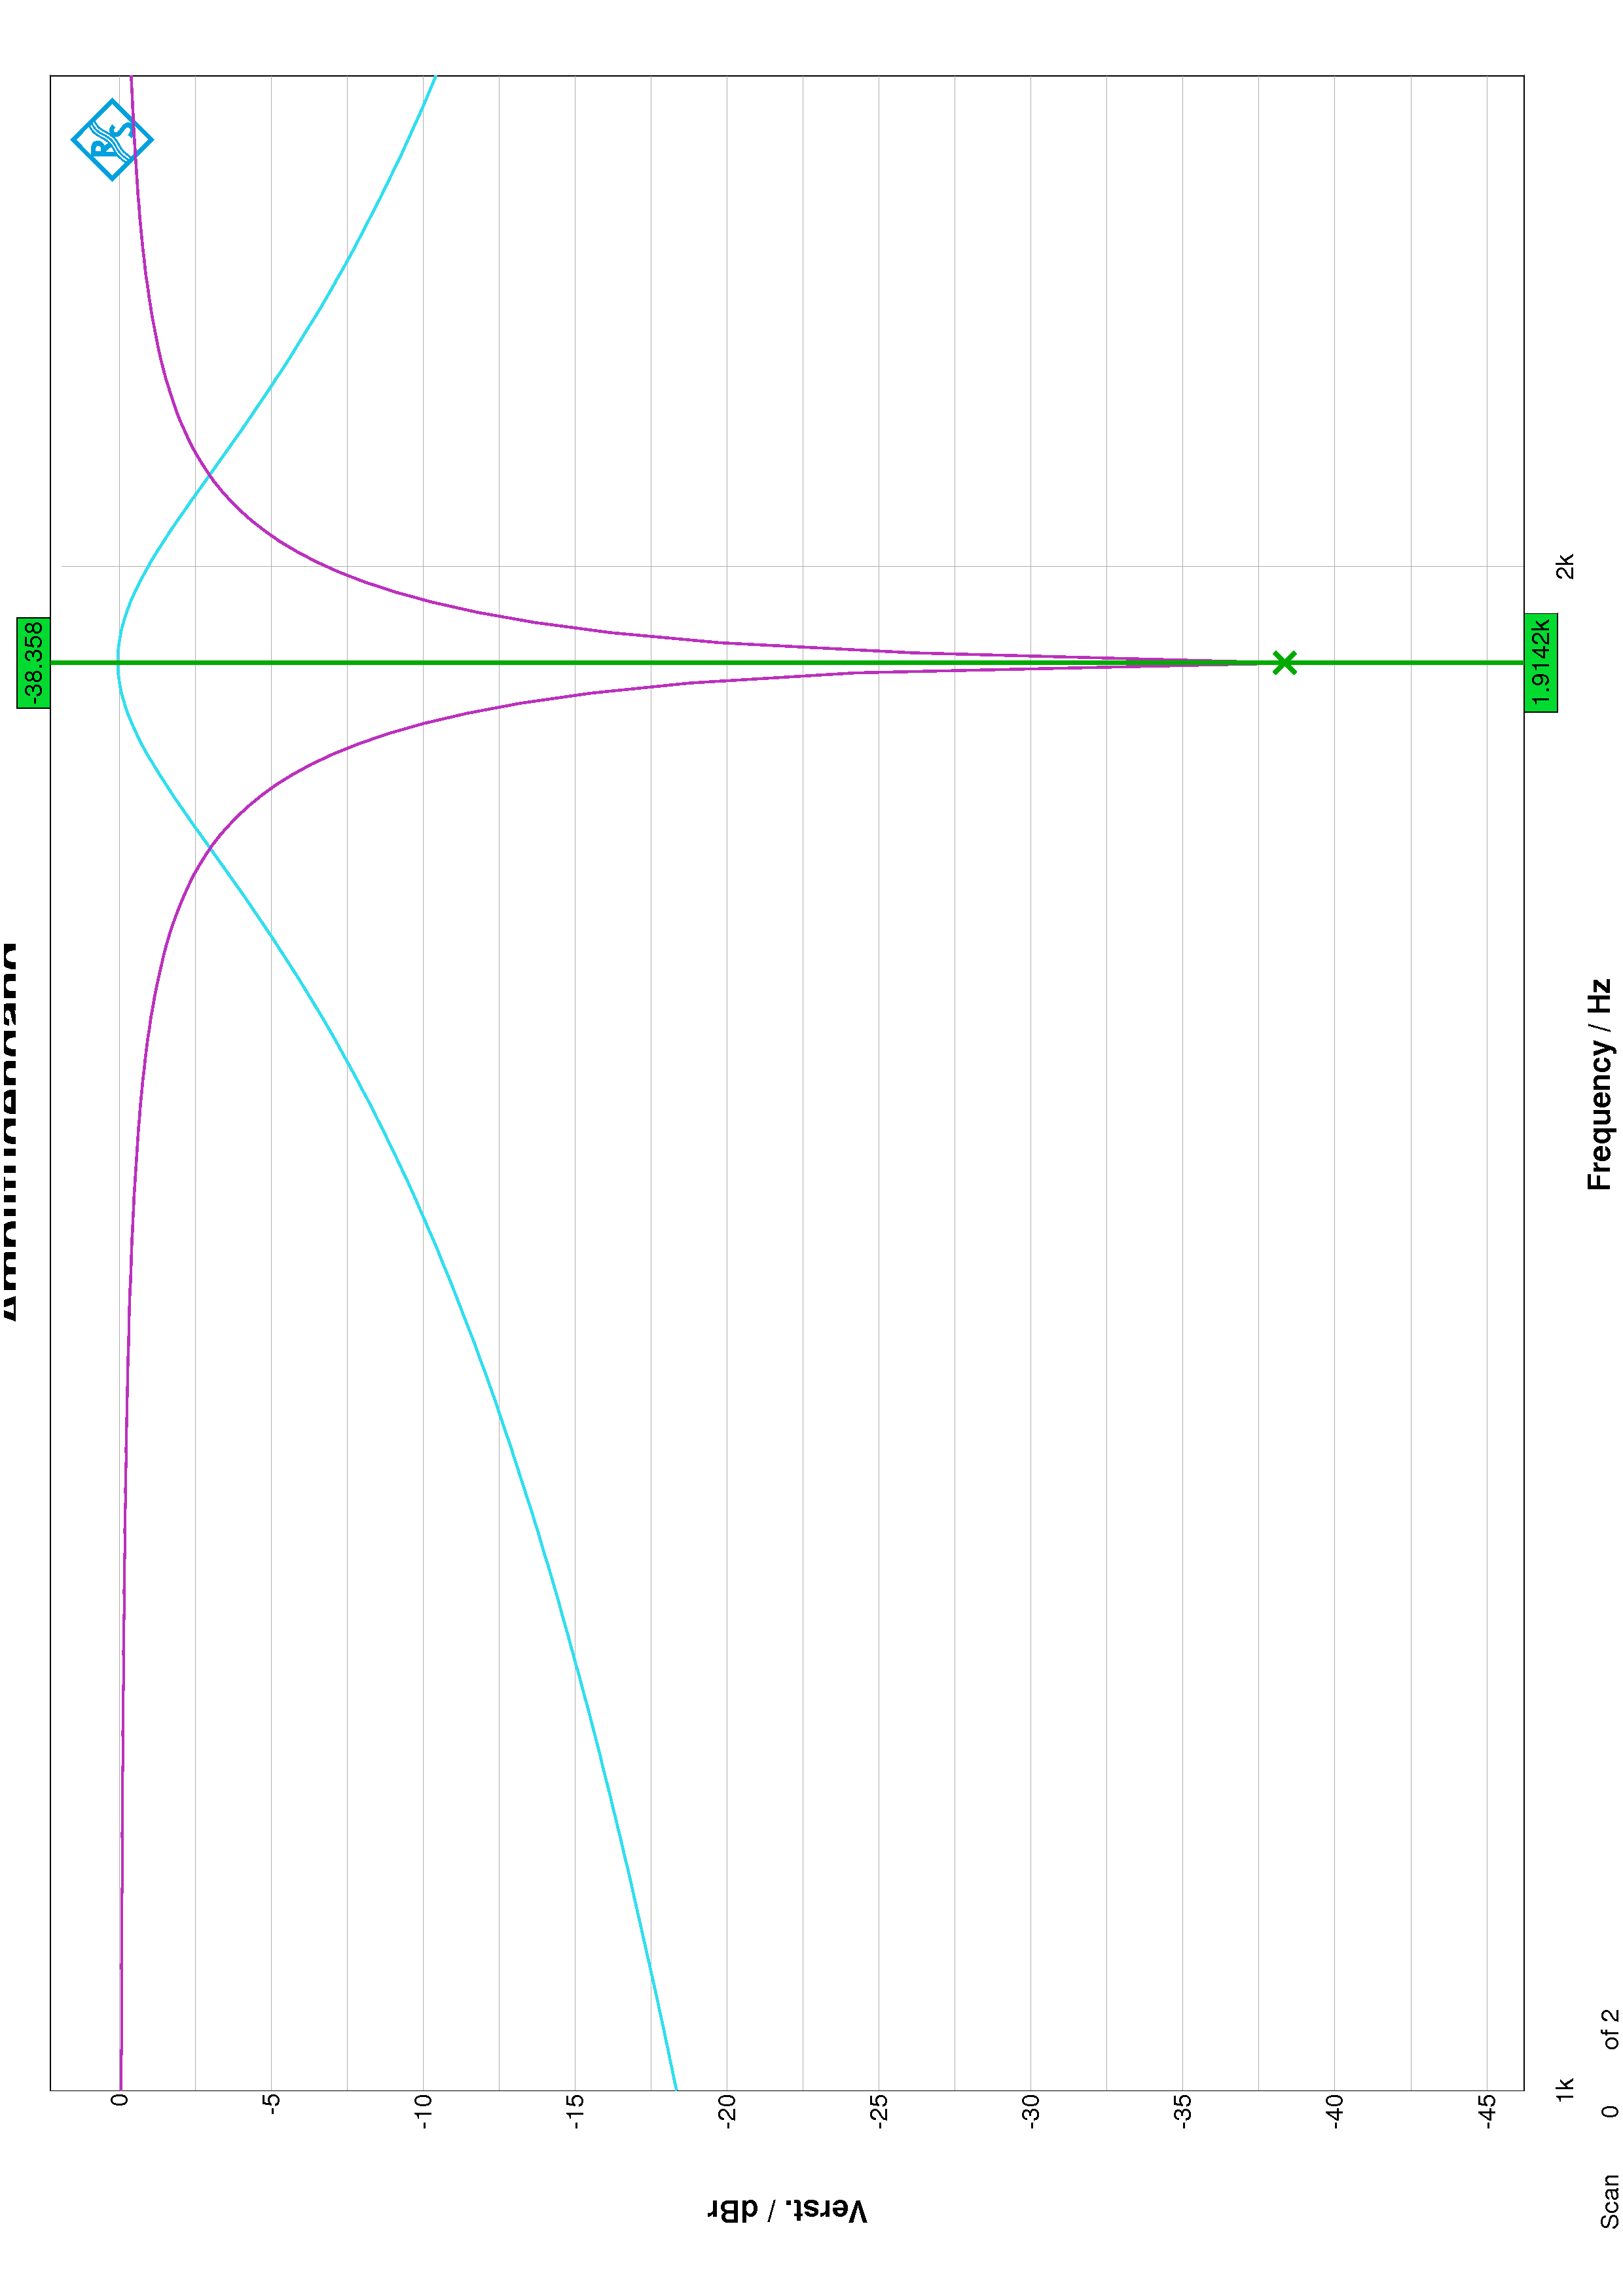
\includegraphics[width = \textwidth/3, angle =-90]{img/3.4 Amplitudengang Bandsperre.png}}\\
\subfloat[Bandbreite Bandpass]{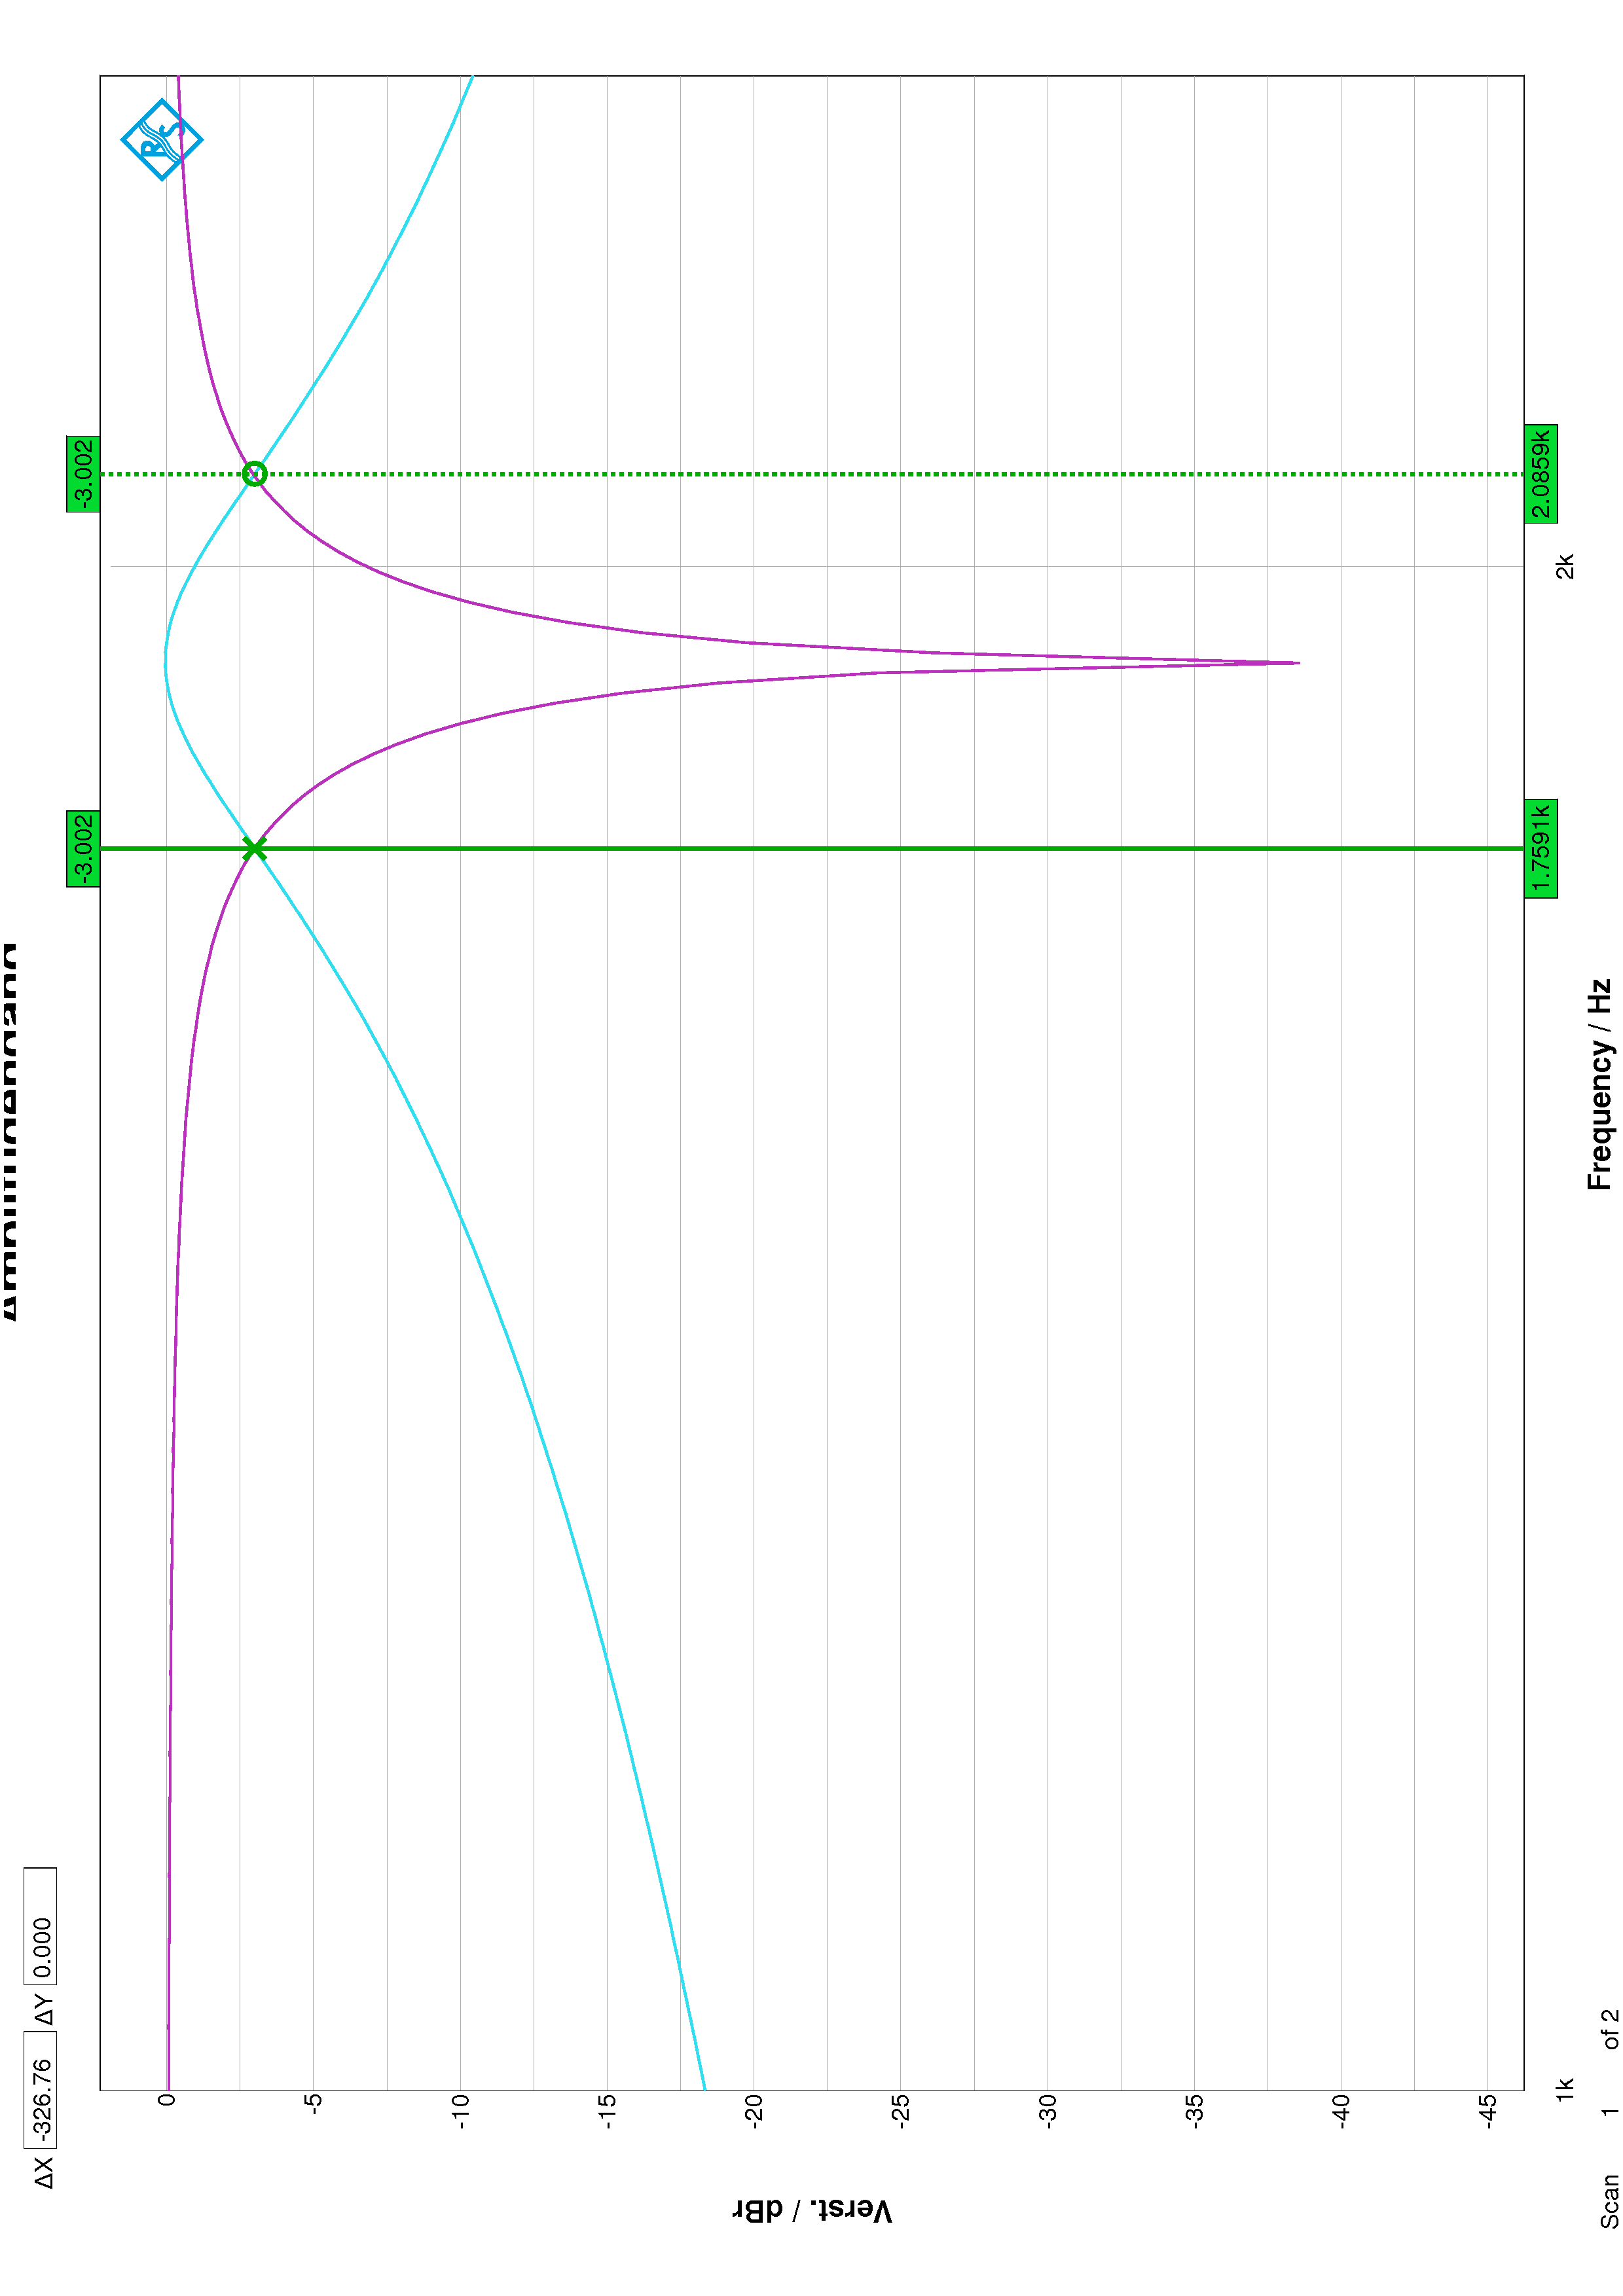
\includegraphics[width = \textwidth/3, angle =-90]{img/3.4 Bandbreite Bandpass.png}} 
\subfloat[Bandbreite Bandsperre]{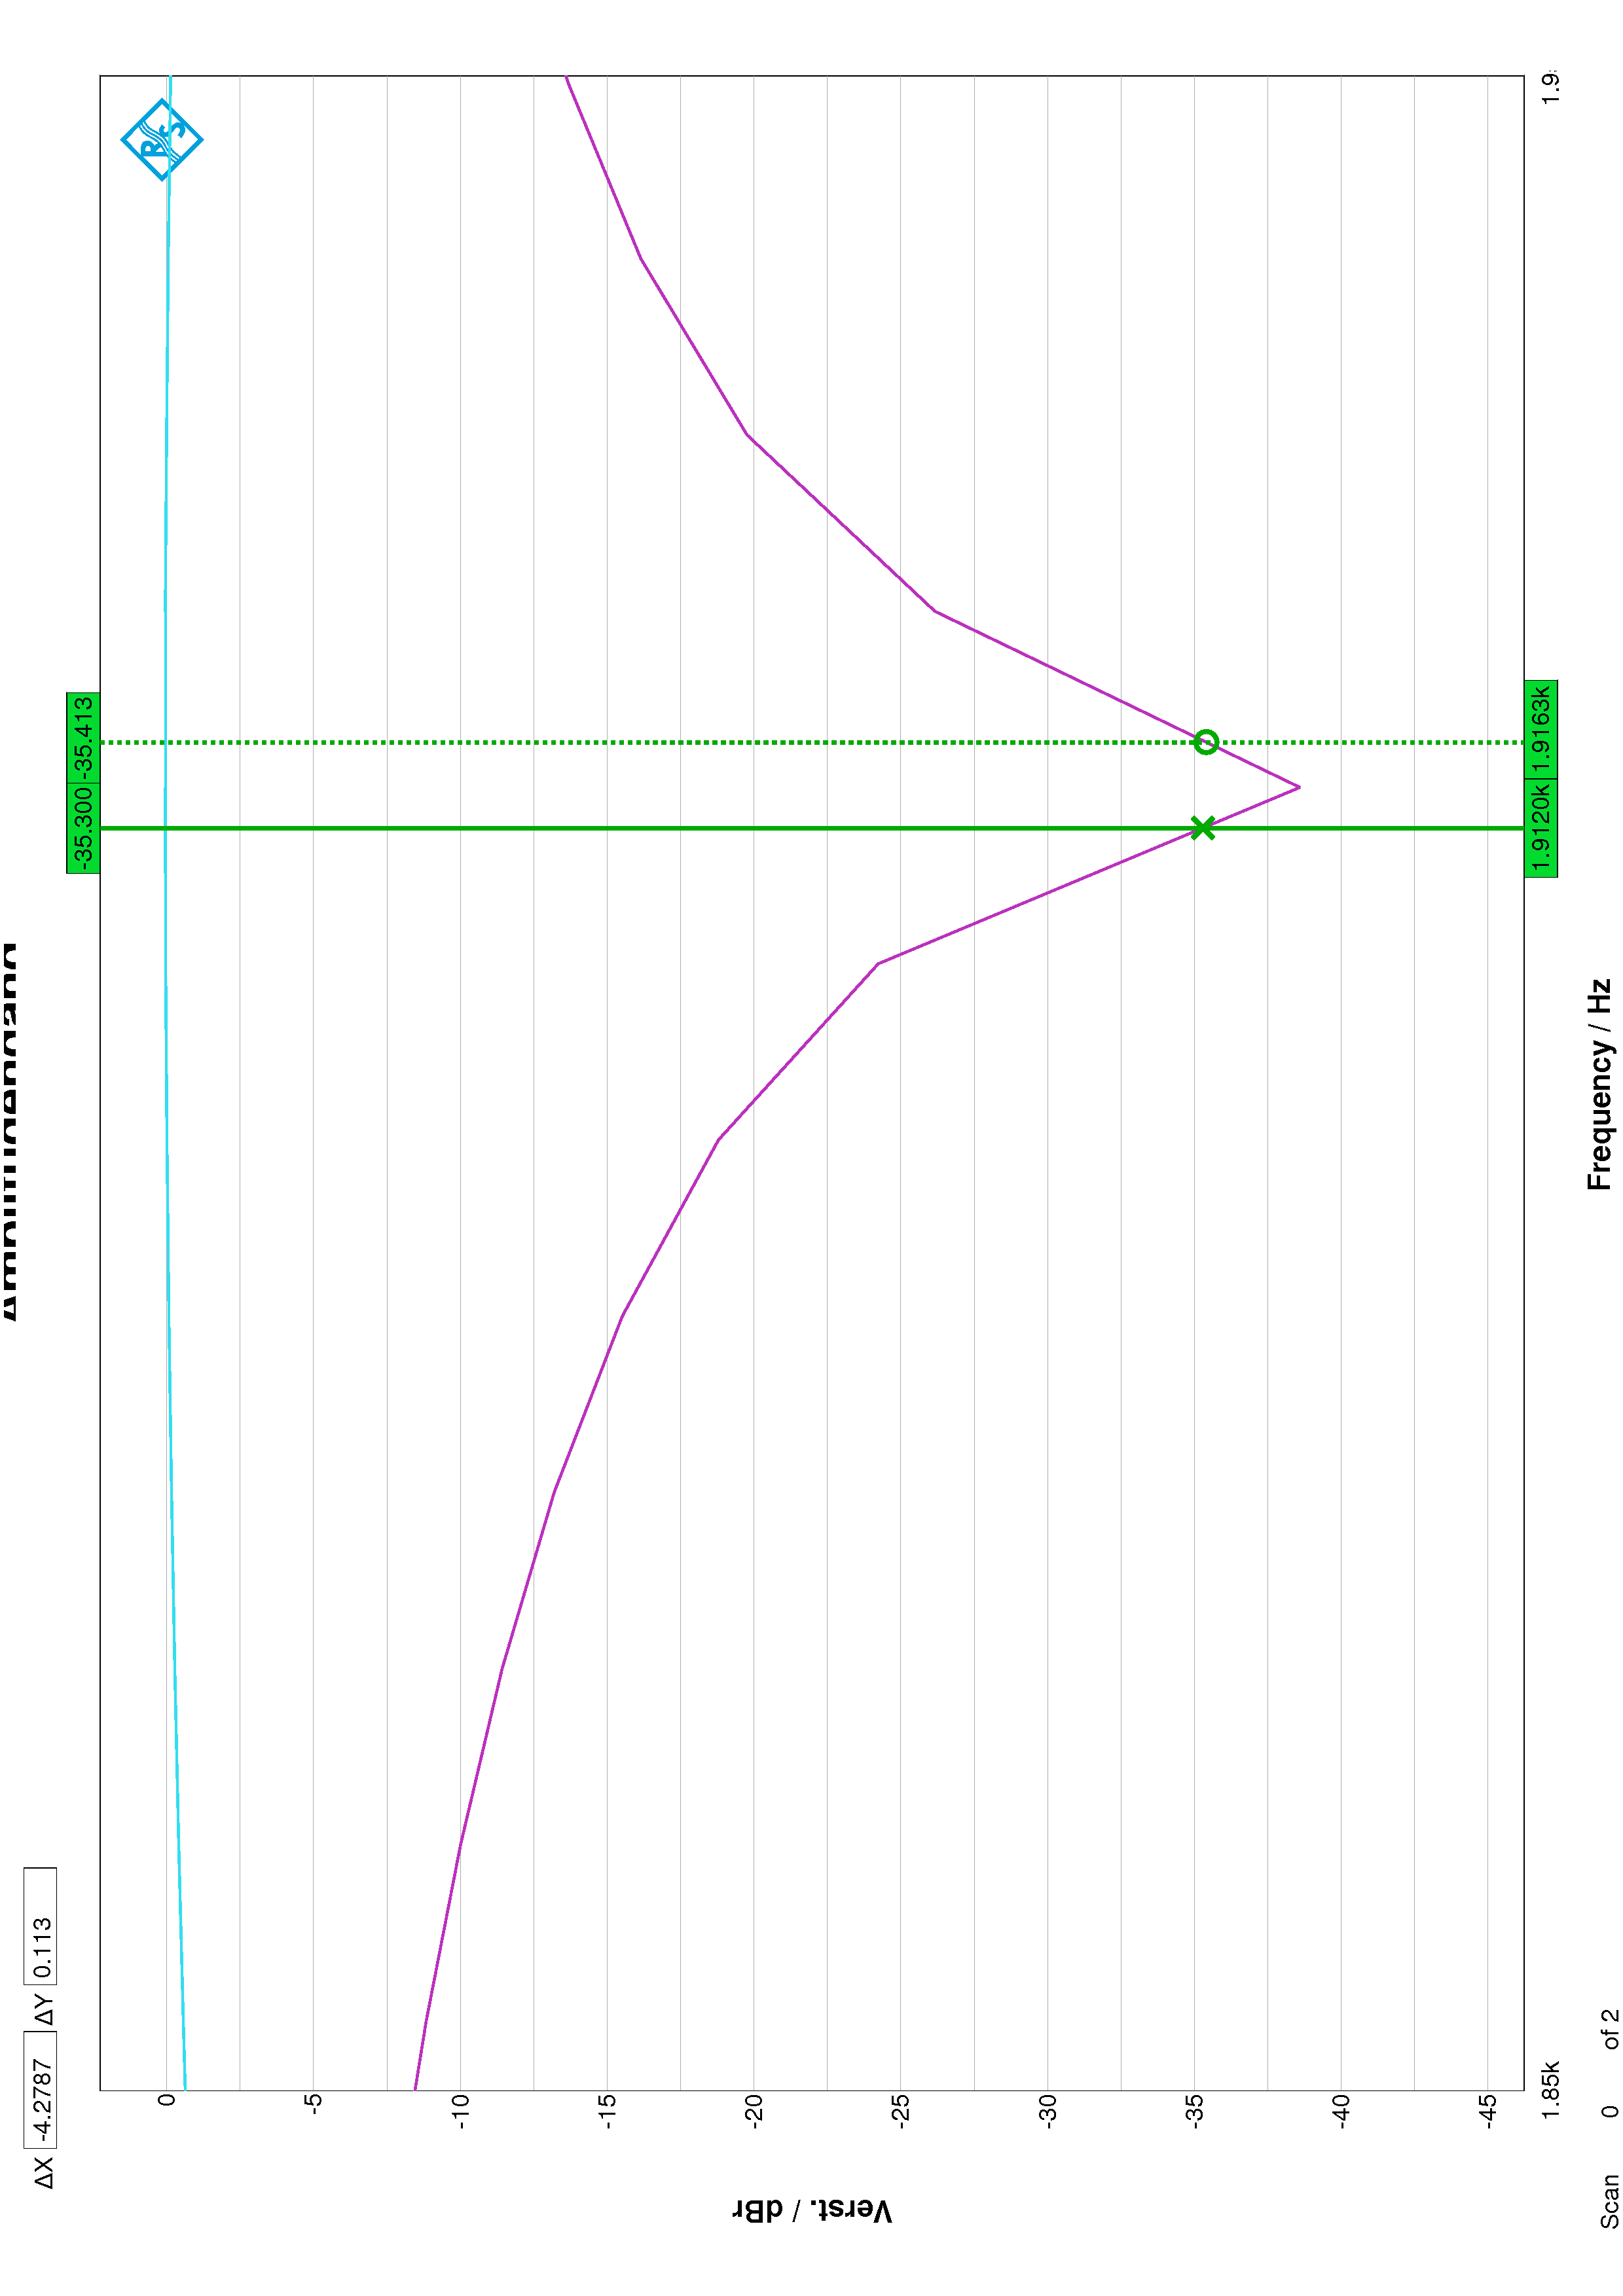
\includegraphics[width = \textwidth/3, angle =-90]{img/3.4 Bandbreite Bandsperre.png}} 
\caption{Bandbreiten}
\label{fig:A3_mult}
\end{center}
\end{figure}


\begin{table}[ht]
    \centering
    \begin{tabular}{|c|c|c|c|}\hline
    \tbf{Filter}     & \tbf{Mitte} & \tbf{$\SI{-3}{\decibel}$ unten} & \tbf{$\SI{-3}{\decibel}$ oben} \\ \hline
    Bandpass                   & \SI{1932.3}{\hertz}  & \SI{1759.1}{\hertz} & \SI{2085.9}{\hertz}\\
    Bandsperre                 & \SI{1914.2}{\hertz}  & \SI{1912}{\hertz} & \SI{1916.3}{\hertz}\\ \hline
    \end{tabular}
    \caption{Beispiel Addieren:}
\end{table}






%Amplitudengänge von Butterworth-, Tschebyscheff- und Bessel-Tiefpass und Markierung der Grenzfrequenzen Phasengänge von Butterworth-, Tschebyscheff- und Bessel-Tiefpass und Markierung der Frequenzen für eine Phasenverschiebung von -60° und -120° Amplitudengänge von Butterworth-, Tschebyscheff- und Bessel-Hochpass und Markierung der Grenzfrequenzen Amplitudengänge von Bandpass und Bandsperre und Markierung der Grenzfrequenzen Auswertung: Alle Messwerte der Grenzfrequenzen sind in einer Tabelle mit den Vorgabewerten einzutragen und zu vergleichen; Aus den Frequenzen bei 60° und 120° Phasenverschiebung sind die Koeffizienten a1, b1 der 3 Tiefpässe zu berechnen und mit den Vorgabewerten zu vergleichen 





















\subsection{Auswertung}
%%%%%%%%%%%%%%%%%%%%%%%%%%%%%%%%%%%%%%%%%%%%%%%%Comments
%Amplitudengänge von Butterworth-, Tschebyscheff- und Bessel-Tiefpass und Markierung der Grenzfrequenzen Phasengänge von Butterworth-, Tschebyscheff- und Bessel-Tiefpass und Markierung der Frequenzen für eine Phasenverschiebung von -60° und -120° Amplitudengänge von Butterworth-, Tschebyscheff- und Bessel-Hochpass und Markierung der Grenzfrequenzen Amplitudengänge von Bandpass und Bandsperre und Markierung der Grenzfrequenzen Auswertung: Alle Messwerte der Grenzfrequenzen sind in einer Tabelle mit den Vorgabewerten einzutragen und zu vergleichen; Aus den Frequenzen bei 60° und 120° Phasenverschiebung sind die Koeffizienten a1, b1 der 3 Tiefpässe zu berechnen und mit den Vorgabewerten zu vergleichen
	\section{Sprung}
Das Zeitverhalten der 3 Tiefpässe soll an Hand der Sprungantworten untersucht werden. Zur Messung der Sprungantwort wird das Filter mit einem periodischen Rechtecksignal geeigneter Amplitude und Frequenz aus einem Funktionsgenerator angesteuert und das Ausgangssignal auf dem Oszilloskop abgebildet.
 Skizzieren Sie die Messschaltung mit Angabe der verwendeten Geräte und plotten Sie Einund Ausgangssignale für die drei Tiefpässe. Bestimmen Sie aus den Sprungantworten der drei Tiefpässe Anstiegszeit, Überschwingen (bezogen auf Endwert) und Einschwingzeit (bezogen auf 5% Abweichung vom Endwert) und stellen Sie alle Werte in einer Tabelle gemeinsam dar!


%%%%%%%%%%%%%%%%%%%%%%%%%%%%%%%%%%%%%%%%%%%%%%%%Comments
%Plots der Sprungantworten der drei Tiefpässe, Bestimmung von Anstiegszeit, Überschwingen und Einschwingzeit; Darstellung und Vergleich in einer Tabelle
%multi figure
\begin{figure}[H]
\begin{center}
\subfloat[\imgfilename]{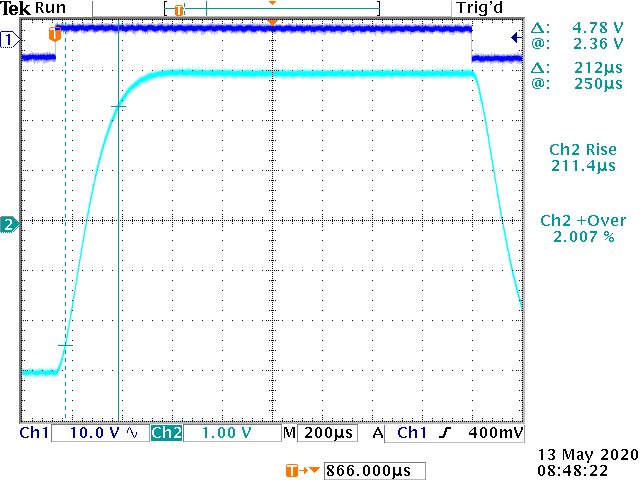
\includegraphics[width = \textwidth/3]{img/4 Bessel Anstiegszeit.png}}  
\subfloat[\imgfilename]{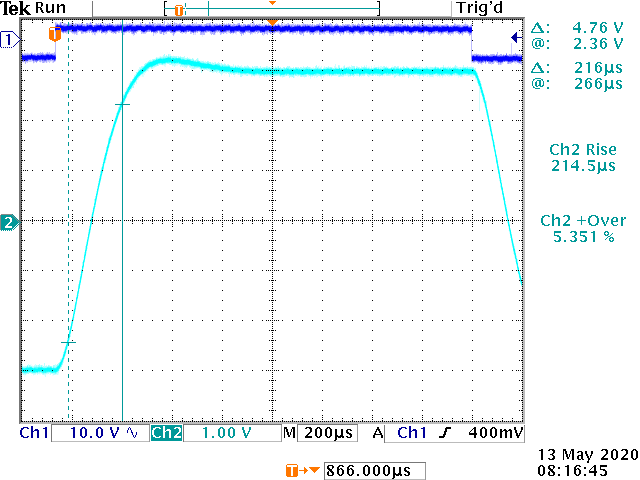
\includegraphics[width = \textwidth/3]{img/4 Butterworth Anstiegszeit .png}} 
\subfloat[\imgfilename]{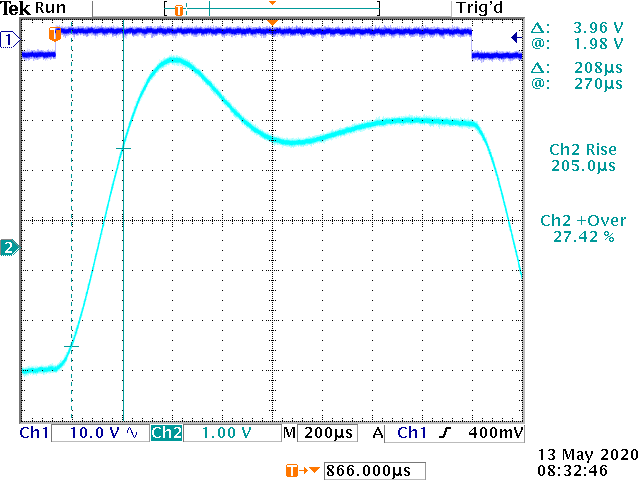
\includegraphics[width = \textwidth/3]{img/4 Tscheby Anstiegszeit.png}} \\
\subfloat[\imgfilename]{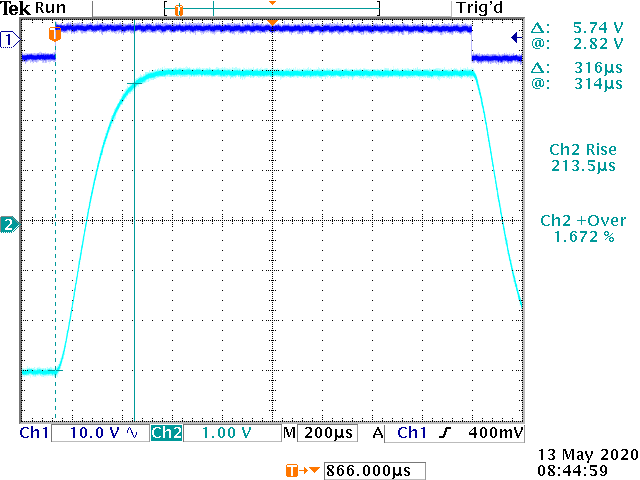
\includegraphics[width = \textwidth/3]{img/4 Bessel Einschwingzeit.png}}  
\subfloat[\imgfilename]{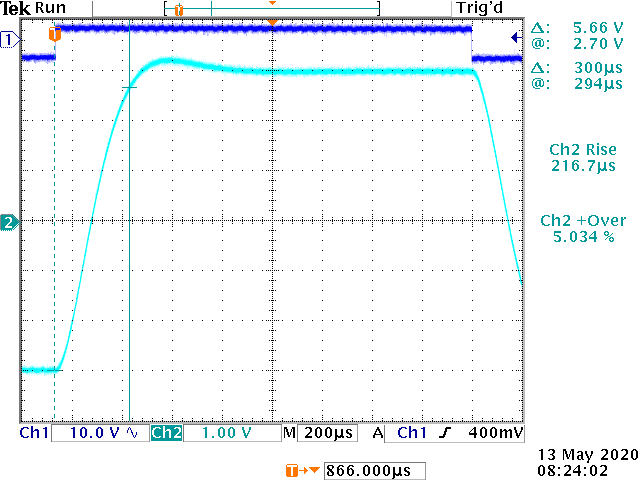
\includegraphics[width = \textwidth/3]{img/4 Butterworth Einschwingzeit.png}} 
\subfloat[\imgfilename]{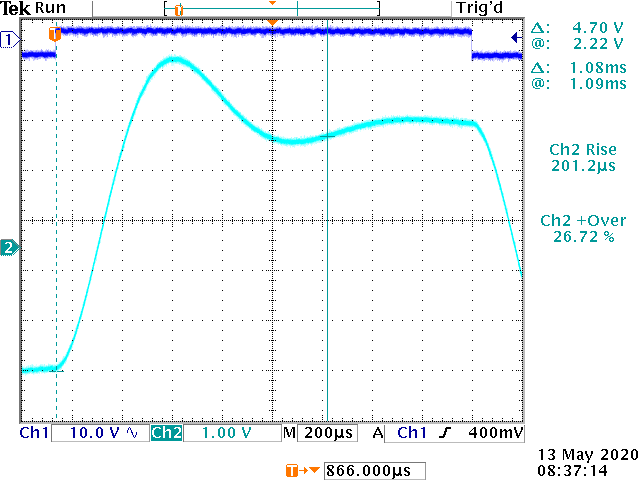
\includegraphics[width = \textwidth/3]{img/4 Tscheby Einschwingzeit.png}} \\
\subfloat[\imgfilename]{\includegraphics[width = \textwidth/3]{img/4 Bessel Überschwingzeit.png}}  
\subfloat[\imgfilename]{\includegraphics[width = \textwidth/3]{img/4 Butterworth Überschwingen}} 
\subfloat[\imgfilename]{\includegraphics[width = \textwidth/3]{img/4 Tscheby Überschwingzeit}} \\
\caption{Anstiegszeit, Einschwingzeit und Überschwingzeit}
\label{fig:A4_mult}
\end{center}
\end{figure}

\begin{table}[H]
    \centering
    \begin{tabular}{|c|c|c|c|c|}\hline
    \tbf{Filter} & \tbf{Anstiegszeit} & \tbf{Überschwingen}     &  \tbf{Einschwingen}     & \tbf{Ausgangsamplitude}   \\ \hline
    Butterworth                   & \SI{216}{\micro\second} &     \SI{0.26}{\volt} &\SI{300}{\micro\second} & \SI{6}{\volt_{pp}}   \\
    Tschebyscheff             & \SI{208}{\micro\second}  &    \SI{1.2}{\volt}  &\SI{1.08}{\milli\second} & \SI{5}{\volt_{pp}}   \\ 
    Bessel                &\SI{212}{\micro\second}  & \SI{40}{\milli\volt} &\SI{316}{\micro\second} &\SI{6}{\volt_{pp}} \\ \hline
    \end{tabular}
    \caption{Grenzfrequenzen der Filter}
\end{table}
	
\section{Auswertung}

	


	\newpage



\end{document}